\documentclass[11pt,titlepage]{jsarticle}
\usepackage{listings}
\usepackage{jlisting}
\usepackage[T1]{fontenc}
\usepackage{textcomp}
\usepackage{ascmac}
\usepackage[dvipdfmx]{graphicx}
\usepackage{array}
\usepackage{float}
\usepackage{moreverb}
\usepackage{framed}

\renewcommand{\lstlistingname}{ソースコード}
\lstset{
  language=c,
  basicstyle=\ttfamily\scriptsize,
  commentstyle=\textit,
  classoffset=1,
  keywordstyle=\bfseries,
  frame=tRBl,
  framesep=5pt,
  showstringspaces=false,
  numbers=left,
  stepnumber=1,
  numberstyle=\tiny,
  tabsize=2,
  breaklines=true
}
\setcounter{page}{1}

\title{シミュレーション}
\author{4年電子情報工学科\\34番 横前洸佑}
\date{提出日:2020/2/18(火)\\	提出期限:2020/2/17(月)10:00}
\begin{document}

\maketitle

\section{課題11}
課題11では、ガウスの消去法を用いて連立方程式(\ref{eq:gauss})を解き、$x_1, x_2, x_3, x_4$を求める。


\begin{eqnarray}
\label{eq:gauss}
		\begin{array}{l}
			x_1 + 2x_2 + x_3 + 5x_4 = 20.5\\
			8x_1 + x_2 + 3x_3 + x_4 = 14.5\\
			x_1 + 7x_2 + x_3 + x_4 = 18.5\\
			x_1 + x_2 + 6x_3 + x_4 = 9.0\\
		\end{array}
\end{eqnarray}

\subsection{作成したプログラム}
今回作成したプログラムをソースコード\ref{src:kadai11}に示す。

\lstinputlisting[caption=課題11のプログラム,label=src:kadai11]{src/kadai11.c}
ガウスの消去法の計算部分を関数として用意し、main関数内から呼び出している。

\subsection{プログラムの実行結果}
実行結果を以下に示す。
\begin{oframed}
\verbatimtabinput[2]{result/kadai11.txt}
\end{oframed}

\subsection{考察}
元の方程式に計算によって得た値を代入する。
\begin{eqnarray}
\label{eq:gauss_result}
		\begin{array}{l}
			1.0 + 2\times2.0 + 0.5 + 5\times3.0 = 20.5\\
			8\times1.0 + 2.0 + 3\times0.5 + 3.0 = 14.5\\
			1.0 + 7\times2.0 + 0.5 + 3.0 = 18.5\\
			1.0 + 2.0 + 6\times0.5 + 3.0 = 9.0\\
		\end{array}
\end{eqnarray}
式がすべて成り立つ。
この結果よりプログラムは正しく動作していると言える。

\section{課題12}
課題12では、ガウスの消去法を用いて連立方程式(\ref{eq:gauss_pivot})を解き、$x_1, x_2, x_3, x_4$を求める。
また、ピボット選択なしで、float型で変数を宣言した場合とdouble型で変数を宣言した場合について解いた時、ピボット選択ありで、float型で変数を宣言した場合とdouble型で変数を宣言した場合について解いた時の結果の違いを考察する。


\begin{eqnarray}
\label{eq:gauss_pivot}
		\begin{array}{l}
			1.0x_1 + 0.96x_2 + 0.84x_3 + 0.64x_4 = 3.44\\
			0.96x_1 + 0.9214x_2 + 0.4406x_3 + 0.2222x_4 = 2.5442\\
			0.84x_1 + 0.4406x_2 + 1.0x_3 + 0.3444x_4 = 2.6250\\
			0.64x_1 + 0.2222x_2 + 0.3444x_3 + 1.0x_4 = 2.2066\\
		\end{array}
\end{eqnarray}

\subsection{作成したプログラム}
今回作成したプログラムをソースコード\ref{src:kadai12}に示す。

\lstinputlisting[caption=課題12のプログラム,label=src:kadai12]{src/kadai12.c}
ガウスの消去法の計算部分を関数として用意し、main関数内から呼び出している。
また、{\tt gauss()}関数内36行目でピボット選択を行う。

\subsection{プログラムの実行結果}
ピボット選択なしで、float型で実行した結果を以下に示す。

\begin{oframed}
\verbatimtabinput[2]{result/kadai12_nonpivot_float.txt}
\end{oframed}

ピボット選択なしで、double型で実行した結果を以下に示す。

\begin{oframed}
\verbatimtabinput[2]{result/kadai12_nonpivot_double.txt}
\end{oframed}

ピボット選択ありで、float型で実行した結果を以下に示す。

\begin{oframed}
\verbatimtabinput[2]{result/kadai12_nonpivot_float.txt}
\end{oframed}

ピボット選択ありで、double型で実行した結果を以下に示す。

\begin{oframed}
\verbatimtabinput[2]{result/kadai12_pivot_double.txt}
\end{oframed}

\subsection{考察}
元の方程式に計算によって得た値を代入する。
\begin{eqnarray}
\label{eq:gauss_pivot_result}
		\begin{array}{l}
			1.0 + 0.96 + 0.84 + 0.64 = 3.44\\
			0.96 + 0.9214 + 0.4406 + 0.2222 = 2.5442\\
			0.84 + 0.4406 + 1.0 + 0.3444 = 2.6250\\
			0.64 + 0.2222 + 0.3444 + 1.0 = 2.2066\\
		\end{array}
\end{eqnarray}
式がすべて成り立つ。
この結果よりプログラムは正しく動作していると言える。

\section{課題13}
表\ref{table:kadai13}に示す7組のデータに対して2次式で近似を行うプログラムを作成する。


\begin{table}[H]
\caption{データ}
\label{table:kadai13}
\centering
\begin{tabular}{|c|c|c|c|c|c|c|c|}\hline
	$i$&1&2&3&4&5&6&7 \\ \hline
	$x_i$&0.0&0.1&0.2&0.3&0.4&0.5&0.6 \\ \hline
	$y_i$&0.000&0.034&0.138&0.282&0.479&0.724&1.120\\ \hline
\end{tabular}
\end{table}


\subsection{作成したプログラム}
今回作成したプログラムをソースコード\ref{src:kadai13}に示す。

\lstinputlisting[caption=課題13のプログラム,label=src:kadai13]{src/kadai13.c}

\subsection{プログラムの実行結果}
プログラムの実行結果を以下に示す。
\begin{oframed}
\verbatimtabinput[2]{result/kadai13.txt}
\end{oframed}


$y=a+bx+cx^2$ の場合、a=0.008333, b=-0.0575, c=3.1202となっているため正しく動作している。

\section{課題14-1}
1次元ランダムウォークのシミュレーションを行うプログラムを作成する。
なお右へ動く確率を、p=0.5の場合と、p=0.7の場合について計算する。

\subsection{作成したプログラム}
今回作成したプログラムをソースコード\ref{src:kadai14-1}に示す。

\lstinputlisting[caption=課題14-1のプログラム,label=src:kadai14-1]{src/kadai14_1.c}

\subsection{プログラムの実行結果}
p=0.5の場合のプログラムの実行結果を以下に示す。
\begin{oframed}
\verbatimtabinput[2]{result/kadai14_1_05.txt}
\end{oframed}

p=0.7の場合のプログラムの実行結果を以下に示す。
\begin{oframed}
\verbatimtabinput[2]{result/kadai14_1_07.txt}
\end{oframed}

\subsection{考察}
p=0.5の場合において、横軸をステップ数、縦軸を分散とし、分散のデータ値、一次直線、二次曲線を同一のグラフにプロットすると、図\ref{fig:kadai14_1_05}のようになる。

\begin{figure}[H]
\centering
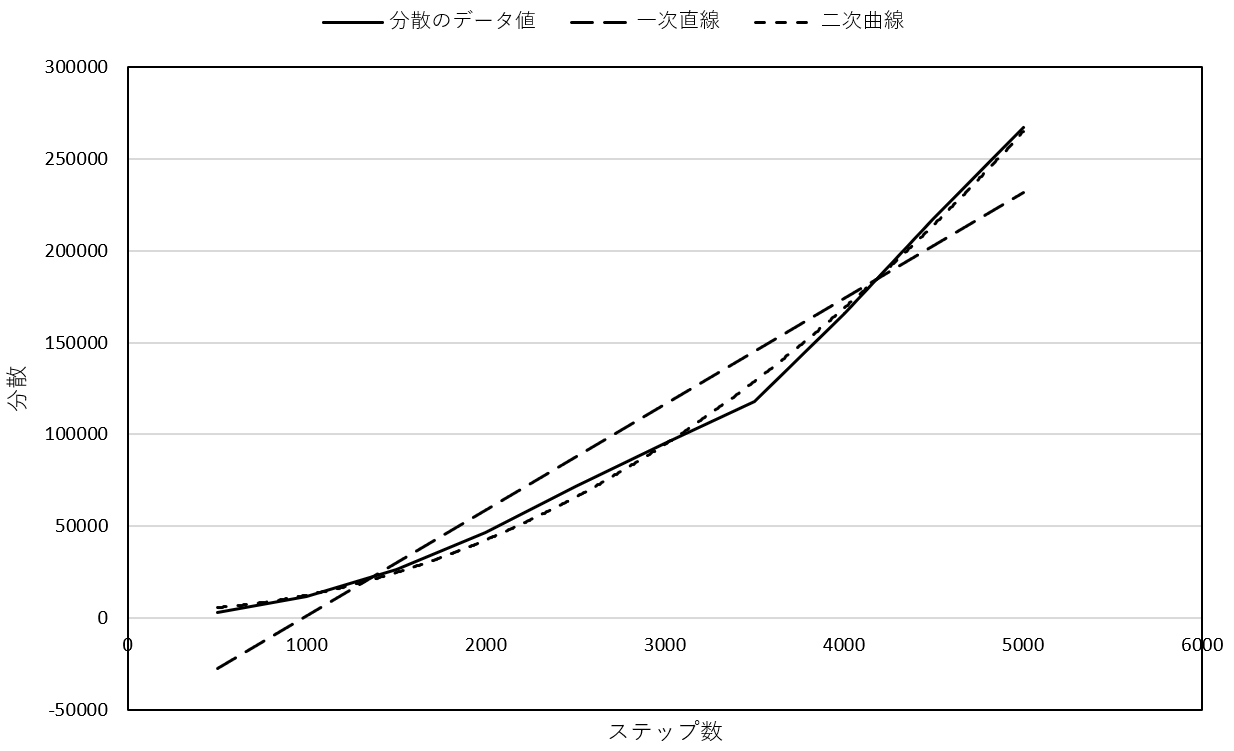
\includegraphics[width=12cm]{img/kadai14_1_05.PNG}
\caption{$p=0.5$の場合}
\label{fig:kadai14_1_05}
\end{figure}

グラフより、単調増加していることがわかる。

p=0.7の場合においてグラフをプロットすると、図\ref{fig:kadai14_1_07}のようになる。

\begin{figure}[H]
\centering
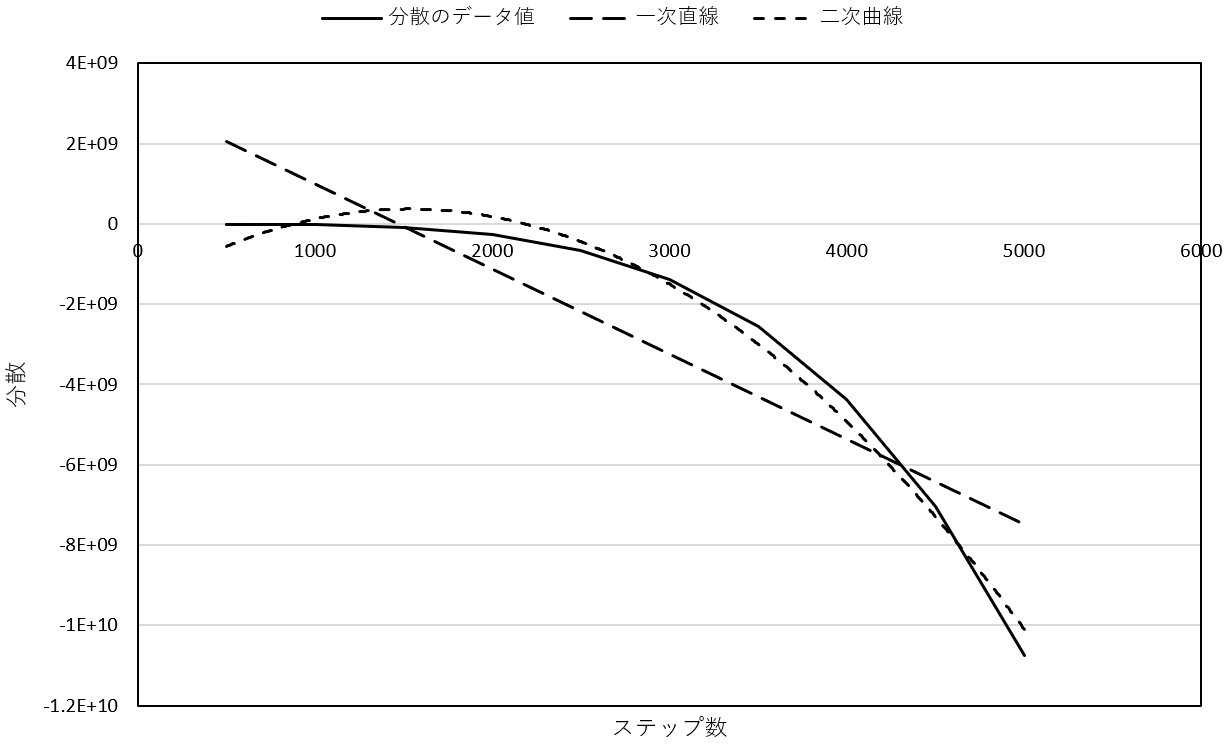
\includegraphics[width=12cm]{img/kadai14_1_07.PNG}
\caption{$p=0.7$の場合}
\label{fig:kadai14_1_07}
\end{figure}

グラフより、分散は急激に減少することがわかる。


\section{課題14-2}
2次元ランダムウォークのシミュレーションを行うプログラムを作成する。
粒子を200個用意し、Nステップ後にどのような模様になるか調べる。
今回は、N=500とする。

\subsection{作成したプログラム}
今回作成したプログラムをソースコード\ref{src:kadai14-2}に示す。

\lstinputlisting[caption=課題14-2のプログラム,label=src:kadai14-2]{src/kadai14_2.c}

\subsection{プログラムの実行結果}
プログラムの実行結果を以下に示す。なお、量が多いため、一部のみを掲載する。
\begin{oframed}
\verbatimtabinput[2]{result/kadai14_2.txt}
\end{oframed}

\subsection{考察}
各粒子を配置すると図\ref{fig:kadai14_2}のようになる。

\begin{figure}[H]
\centering
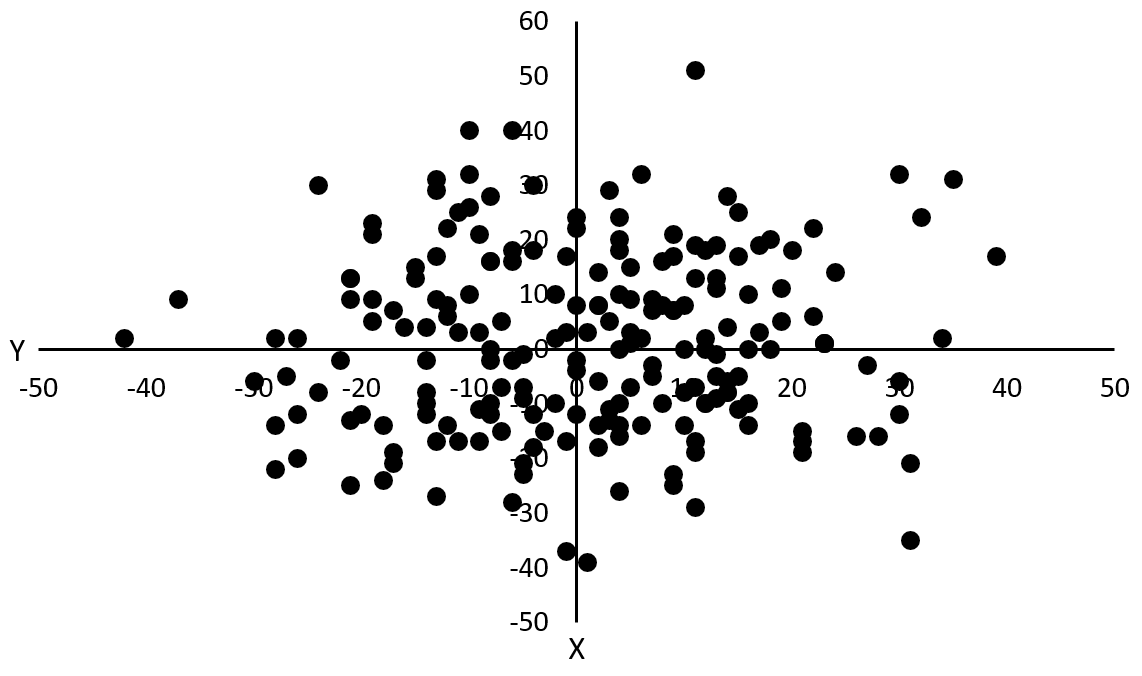
\includegraphics[width=12cm]{img/kadai14_2.PNG}
\caption{各粒子の様子}
\label{fig:kadai14_2}
\end{figure}

各粒子が1匹の蜂と考えた時、蜂の群の境界は、円のようになる。


\end{document}